% Chapter 1

\chapter{绪论}

\section{背景}

每时每刻都有海量的数据在互联网上流动,随着信息革命的深入,各式各样的新技术层出不穷,构建起了一个无比繁荣的互联网生态。但在这繁荣的表象下,别有用心的恶意攻击与日俱增,给人们带来难以估量的巨额损失,网络安全的重要性不断地凸显。



\section{概述}

数据的完整性(integrity)是数据安全、网络安全的重要组成部分。然而一般用户目前在传输文件的时候对此的重视程度不足。例如在网站上下载文件的时候,虽然很多资源提供者同时提供了文件的散列码或数字签名等信息,但在实际使用的过程中很少有用户会在传输完成后主动验证,这就给数据的安全、用户设备的安全造成了一定的隐患。一个可靠的管理系统可以极大程度的帮助用户完成数字签名的验证程序,确保安全性。

\begin{figure}[!htb]
  \centering
  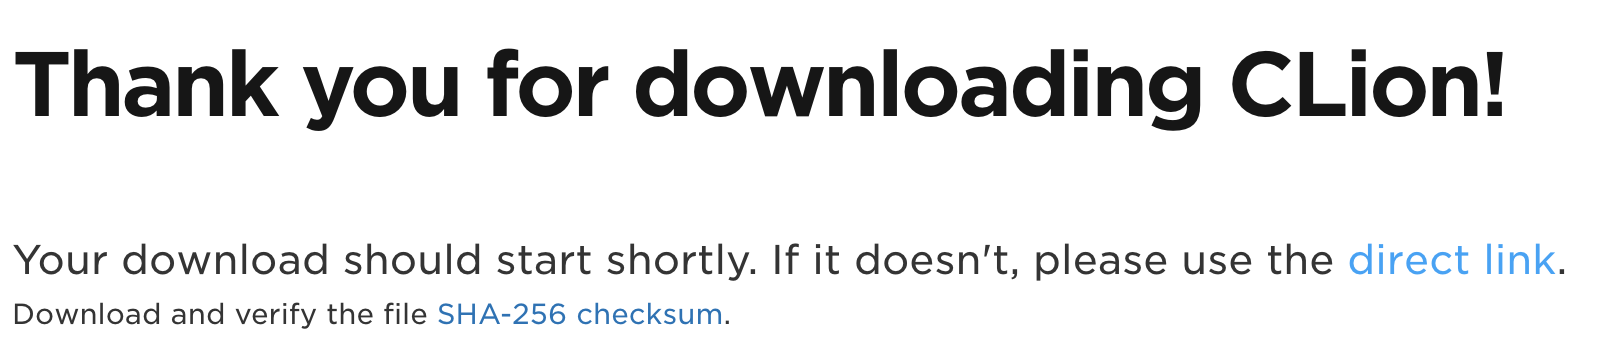
\includegraphics[width=0.7\textwidth]
  {figures/clion.png}\\
  \caption{在下载CLion后官方提供的SHA-256校验和}
  \label{fig:clion}
\end{figure}

本文拟实现一个易于操作、对用户友好的数字签名管理器。在完成以后,成品将以一个完备的网站的形式存在。网站的使用方法简单,页面对用户友好,鲁棒性强,可以直接部署在服务器上。同时项目会很注重安全性,保证程序能够可靠的达成安全地管理数字签名的既定目标。让缺乏专业知识的用户也能正确便捷的管理文件的数字签名。